%# -*- coding: utf-8-unix -*-
%%==================================================
%% motivation.tex for seuthesis Bachelor Thesis
%%==================================================

\chapter{研究动机}
\label{chp:motivation}


\par 过往的很多工作研究了文件被访问热度(skewed file popularities)差别很大的情况下集群缓存系统的负载均衡,在这些工作中,文件复制是被广泛应用的方法。例如,HDFS默认把一份文件复制为3份;当缓存服务器上发生缓存缺失(cache miss),Alluxio弹性增加热门文件在内存中的副本数。

\par 然而文件复制会带来较高的内存开销,最终损害缓存带来的好处。在数据分析的工作中,批处理任务分析结构化数据情况比较多,结构化数据相比一般意义上的文件具有更多的上下文信息,其中列式存储的文件格式,比如Parquet\cite{parquet},得到越来越多的应用,因为在数据分析的大部分任务中,通常需要读取相关列,而不是整行数据,且列式存储把相同类型的数据归在一起,压缩比可以很高。那么问题来了,针对采用列式存储的结构化数据,我们是否能够根据其特有的性质,保证负载均衡的效果的同时,降低文件复制的开销呢?以往的研究工作表明,对一小部分热门文件(被高频访问的文件)访问占据了集群总访问量的大部分,我们猜想,那么对于结构化数据来说,例如具体一张数据表,列与列之间是否存在热门程度的差异呢?如果猜想成立,直观上来说,对于一张表,我们可以只复制最热门的几列,就能达到接近复制全表的负载均衡效果,同时能够降低缓存开销。

\par 如果按照上文所述,仅复制最热门的若干列,缓存在不同的机器上,那么在执行分布式SQL任务的时候,极有可能发生表内部的数据shuffle,我们需要探究shuffle对任务执行时间的影响。直观上来说,数据shuffle带来网络通信上的开销,会降低任务执行的效率,那么在考虑被复制的列在集群里的放置策略时,我们也需要考虑列与列之间被共同访问的概率,如果两列有很大可能性会被一起访问,那么可以考虑将它们“捆绑”(bundle)在一起放置。

\par 在本章~\ref{sec:col-access}节中,我们通过对标准基准数据集TPC系列的分析,来证明数据表中列与列之间,被访问频率存在差异,并且当考虑两两之间被共同访问的概率,两列各自的被访问频率越高,它们被共同访问的频率也越高。在~\ref{sec:data-shuffle}节中,我们通过实验证明数据shuffle会对SQL任务的执行会显著降低任务的执行效率。

\section{列的访问规律}
\label{sec:col-access}

\par 首先我们研究了具有代表性的基准标准测试程序TPC系列中的TPC-H,TPC-DS,TPC-xBB中的列的访问规律。

\subsection{实验设置}

\par 我们通过2.4.0版本的Spark SQL执行三种标准测试程序提供的查询任务。对于每一种,我们生成1 GB\footnote{这个实验与数据量无关,因为数据表的个数和每个表的访问规律不回随着表的规模而改变}的数据,数据存为Parquet格式,然后将查询任务依次提交。三种标准测试程序各自包含的数据表的数量和查询任务的数量总结在表格~\ref{tab:setup}中。当执行查询任务的时候,我们记录对列的访问数据,以此来分析列级别的数据访问的性质。我们从结果中观察到以下两个现象。

\begin{figure}[t]
	\centering
	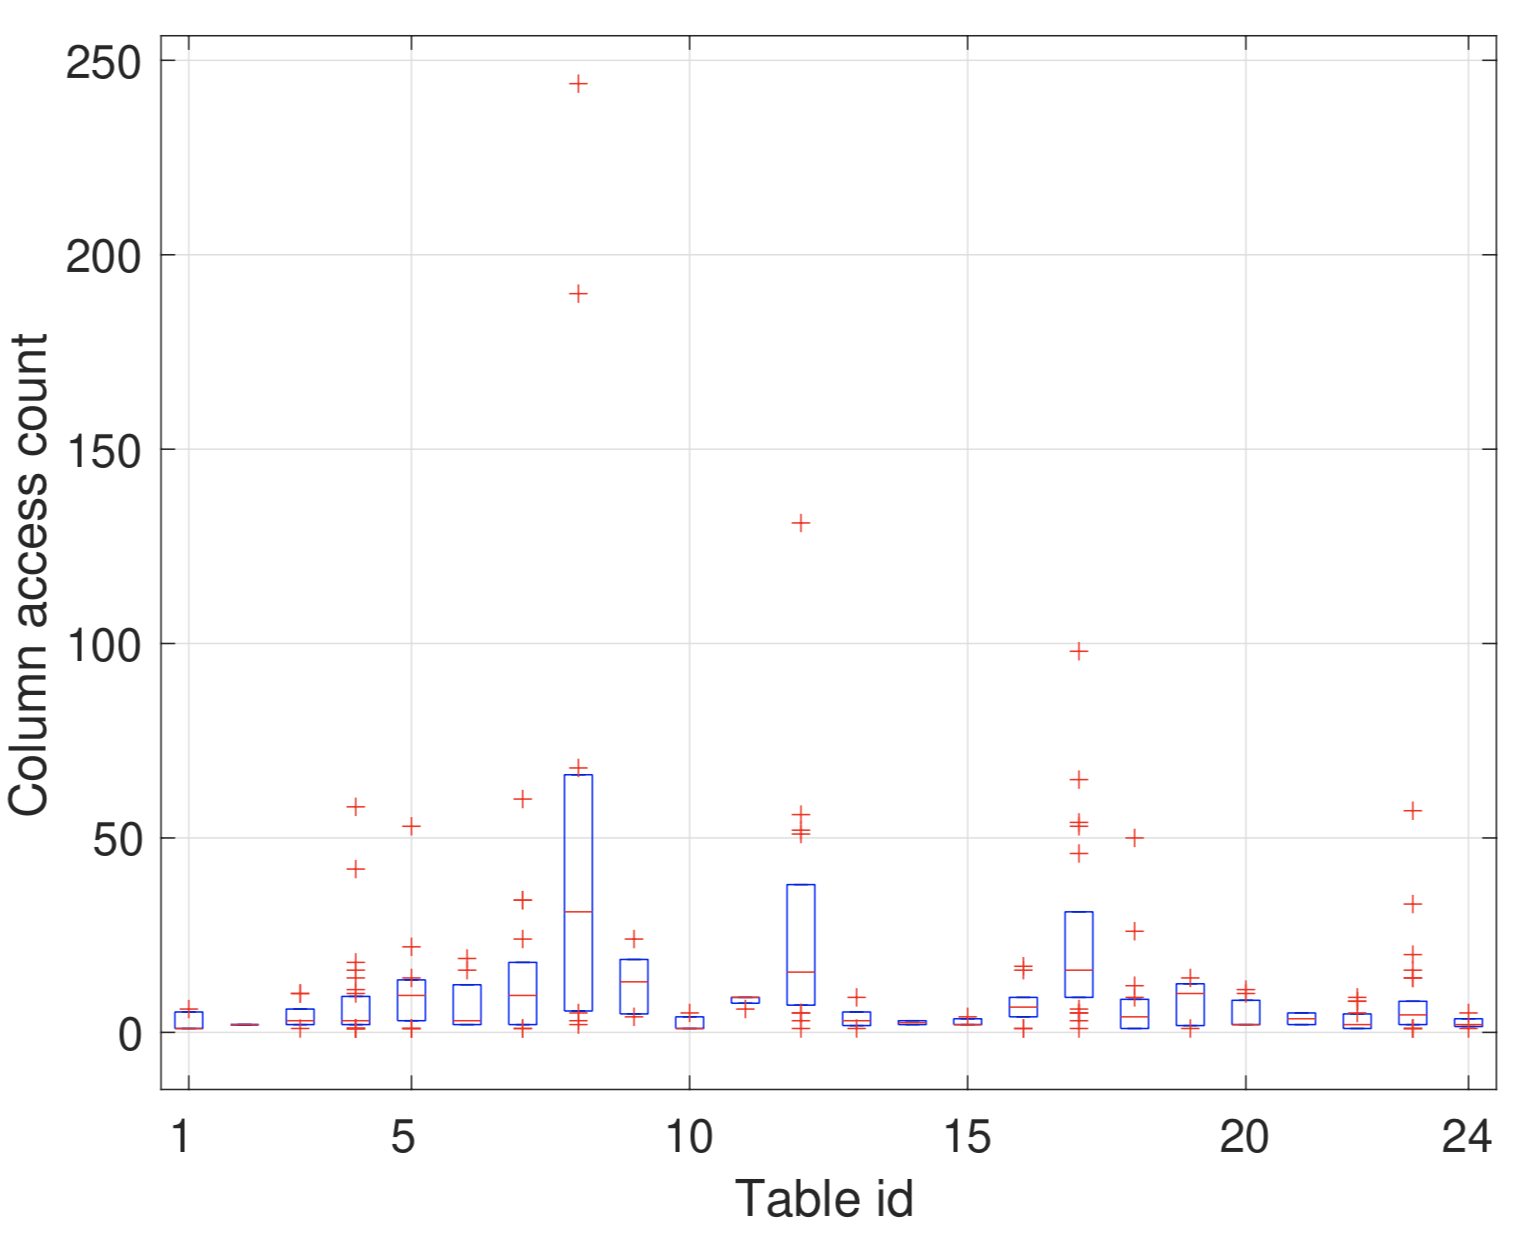
\includegraphics[width=0.5\textwidth]{img/motivation/column-pop}
	\caption{TPC-DS标准测试程序中所有数据表的列访问计数的分布。箱形图展示了每张数据表里$25$\textsuperscript{th}分位,中位数和$75$\textsuperscript{th}分位的列访问次数计数。红色标记表示离群值。}
	\label{fig:tpc-ds-column-pop}
	%\vspace{-.1in}
\end{figure}

\subsection{文件内列访问频率偏差}

\par 在上述三种标准测试程序中,我们观察到,每张数据表内,列的访问频率存在显著差异,即每张表里只有一小部分列被经常访问,而其他的列访问频次比较低。为证明这点,我们对三种标准测试程序中各数据表的列的访问进行了计数。图~\ref{fig:tpc-ds-column-pop}展示了TPC-DS标准测试程序中每张表中列访问计数的分布,箱形图展示了每张数据表里$25$\textsuperscript{th}分位,中位数和$75$\textsuperscript{th}分位的列访问次数计数。每个红色标记表示异常值,特别地,在箱形图上方的红色标记代表该表中访问频率特别高的列。从图上可以看出,对于TPC-DS的多数表,箱形图上方的红色标记远远高于箱形图顶部,这些“热门”的列被访问的次数远远超过均值,这说明文件内列访问频率存在显著偏差。此外,对于各个表而言,表越“热门”(它的列整体上访问频率高),列之间访问频率的差异越大。

\begin{table}[tbp]
    \centering
    \caption{三种标准测试程序的数据}
      \begin{tabularx}{.5\textwidth}{|l|X|X|X|r|}
      \hline
      \textbf{标准测试程序} & \textbf{表的数量} & \textbf{查询任务的数量}  \bigstrut\\ %
      \hline
      TPC-DS & 24  & 99 \bigstrut\\ %
      \hline
      TPC-H & 8  & 22 \bigstrut\\ %
      \hline
      TPC-xBB & 19  & 30 \bigstrut\\ %
      \hline
      \end{tabularx}%
      %\end{tabularx}
    \label{tab:setup}
\end{table}


\par 相似的性质也能在另外两种标准测试程序中看到,图~\ref{fig:count-cdf}展示了三种基准测试程序中所有列的访问计数的总体分布。我们发现,多数的列是“冷门的”,有很多列的访问次数是1,甚至是0,这在TPC-DS(图~\ref{fig:ds-count-cdf})和TPC-xBB(图~\ref{fig:bb-count-cdf})中表现比较明显,而一小部分列有非常高的访问计数。例如,在TPC-DS中,最“热门”的列被访问了多达$89$次。


\begin{figure}[]
    \centering
    \begin{subfigure}[t]{0.5\textwidth}
        \centering
        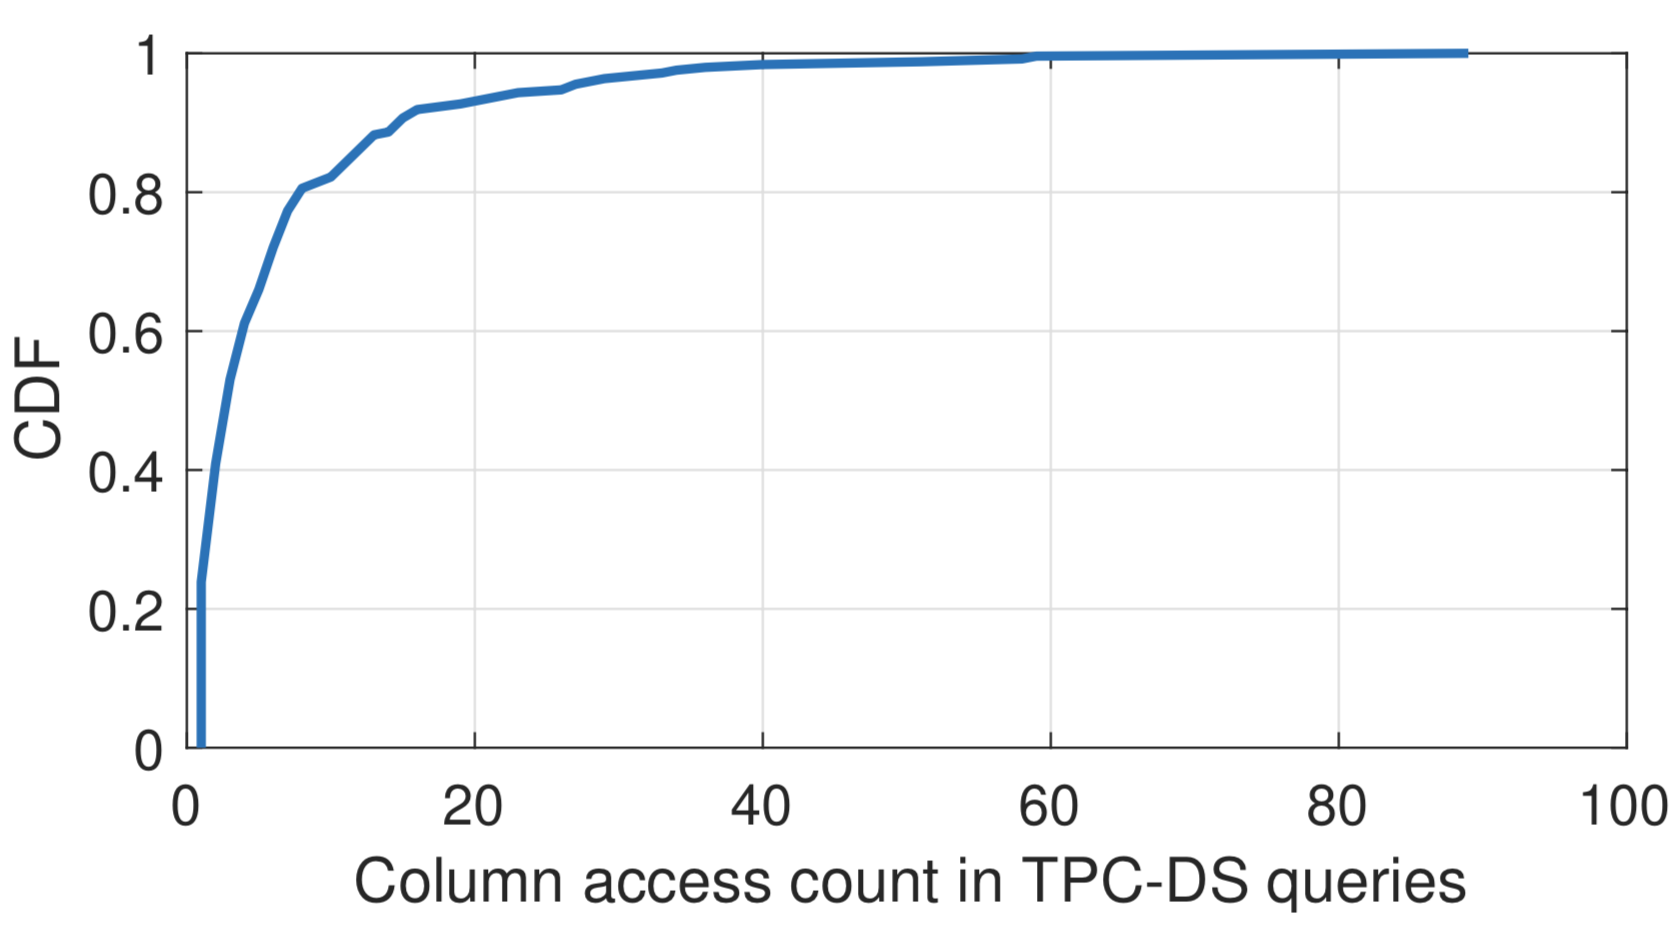
\includegraphics[width=1\textwidth]{img/motivation/ds-count-cdf}
        \caption{TDC-DS.}
        \label{fig:ds-count-cdf}
    \end{subfigure}%

    \begin{subfigure}[t]{0.5\textwidth}
        \centering
        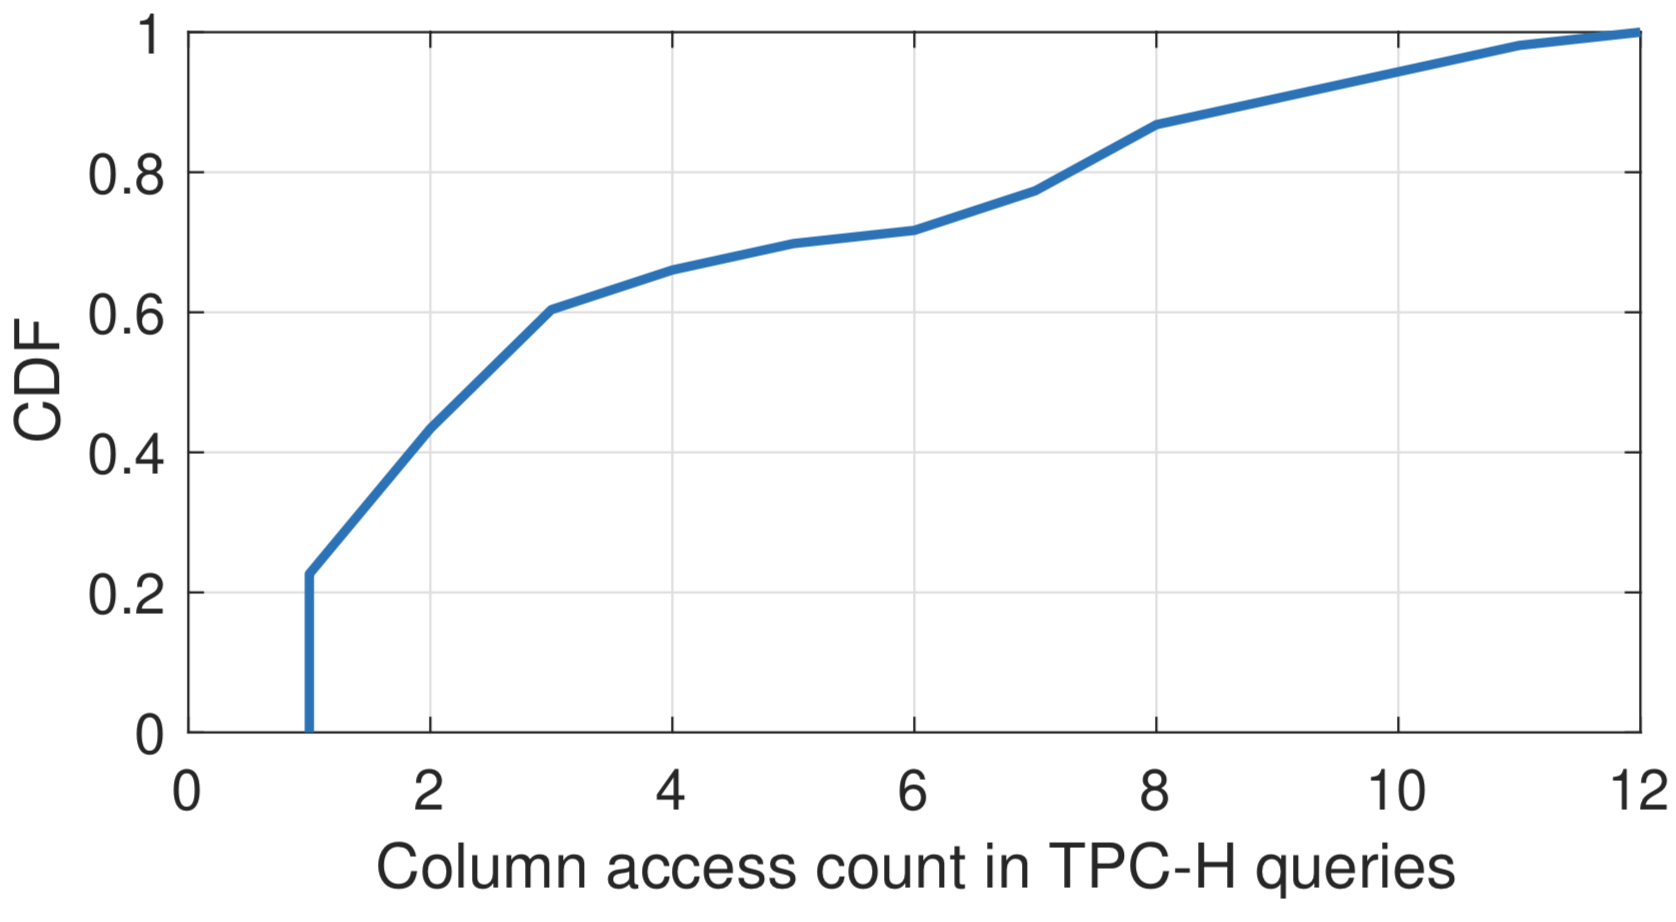
\includegraphics[width=1\textwidth]{img/motivation/h-count-cdf}
        \caption{TDC-H.}
        \label{fig:h-count-cdf}
    \end{subfigure}%

    \begin{subfigure}[t]{0.5\textwidth}
        \centering
        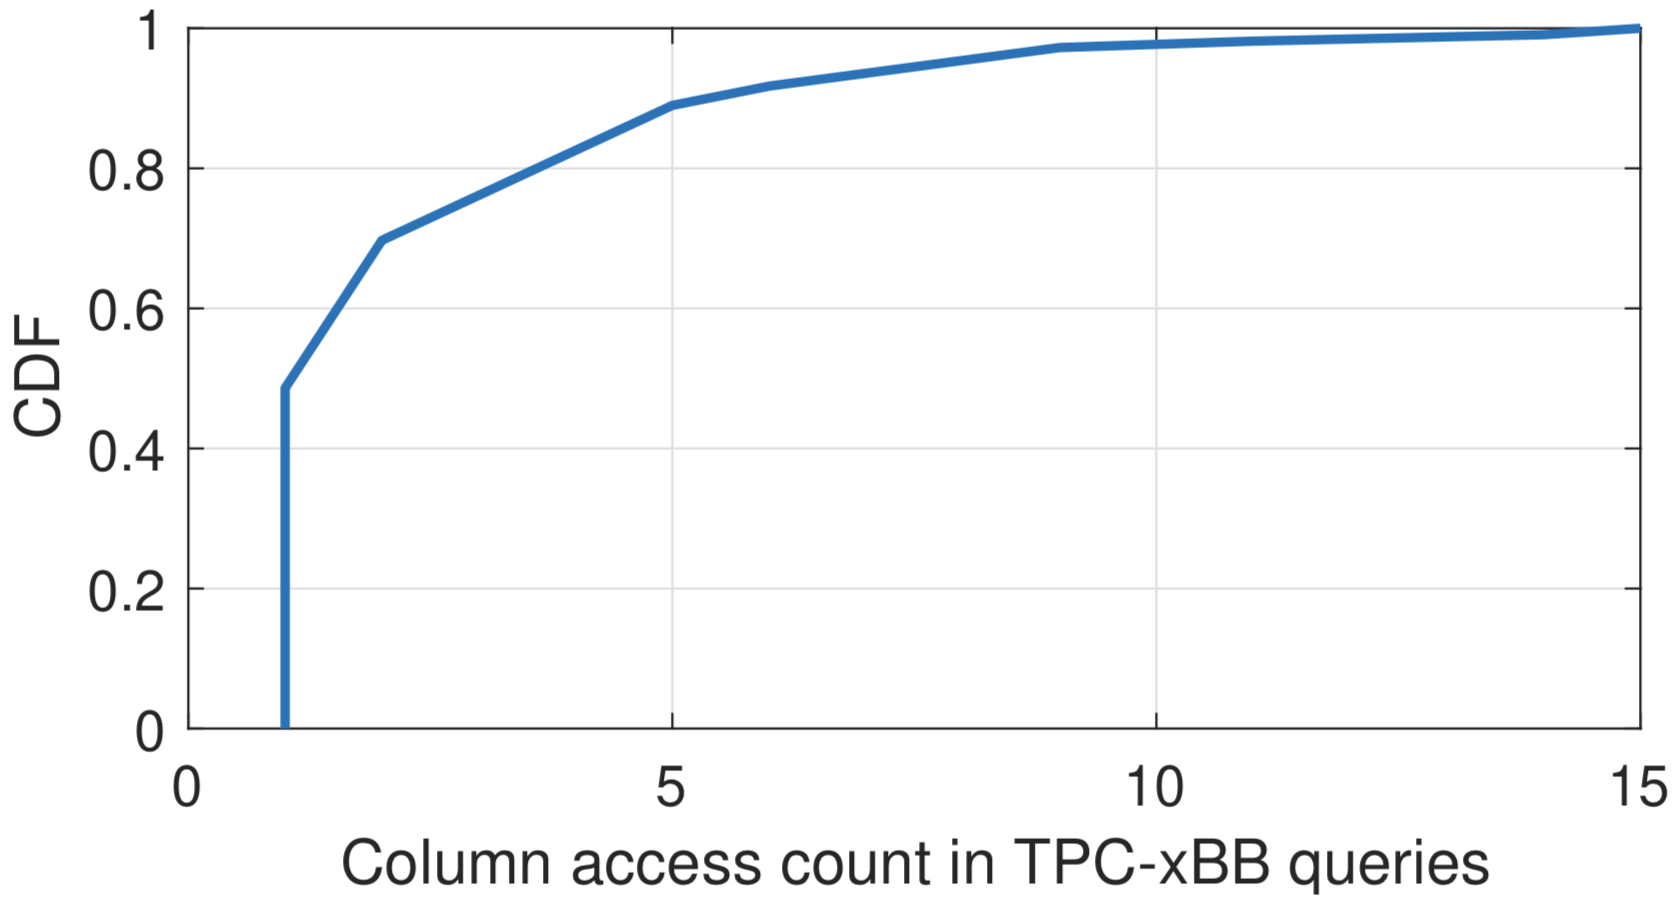
\includegraphics[width=1\textwidth]{img/motivation/xbb-count-cdf}
        \caption{TDC-xBB.}
        \label{fig:bb-count-cdf}
    \end{subfigure}%
    \caption{三种标准测试程序中列访问计数的CDF。}
    \label{fig:count-cdf}
    %\vspace{-.1in}
\end{figure}


\subsection{热门的列被共同访问的规律}
我们观察到的另一个现象是在SQL查询中,“热门”的列有很大概率会被共同访问。为了展示这一点,我们按照列的“热门程度”(访问频次)对列进行排序,绘制访问热图。我们从三个标准测试程序中各选出了一张具有代表性的表,并把结果展示在图~ref{fig:heatmap}中。在热图里,格 $(i,i)$ (也就是对角线上的格子)代表第$i^{th}$热门的列的访问计数,格子$(i,j)$表示第$i^{th}$热门和第$j^{th}$热门的列在同一个查询任务中被共同访问的概率。从图中可以看出,每张表中越是热门的列,被共同访问的概率越高。

\begin{figure}[]
    \centering
    \begin{subfigure}[t]{0.5\textwidth}
        \centering
        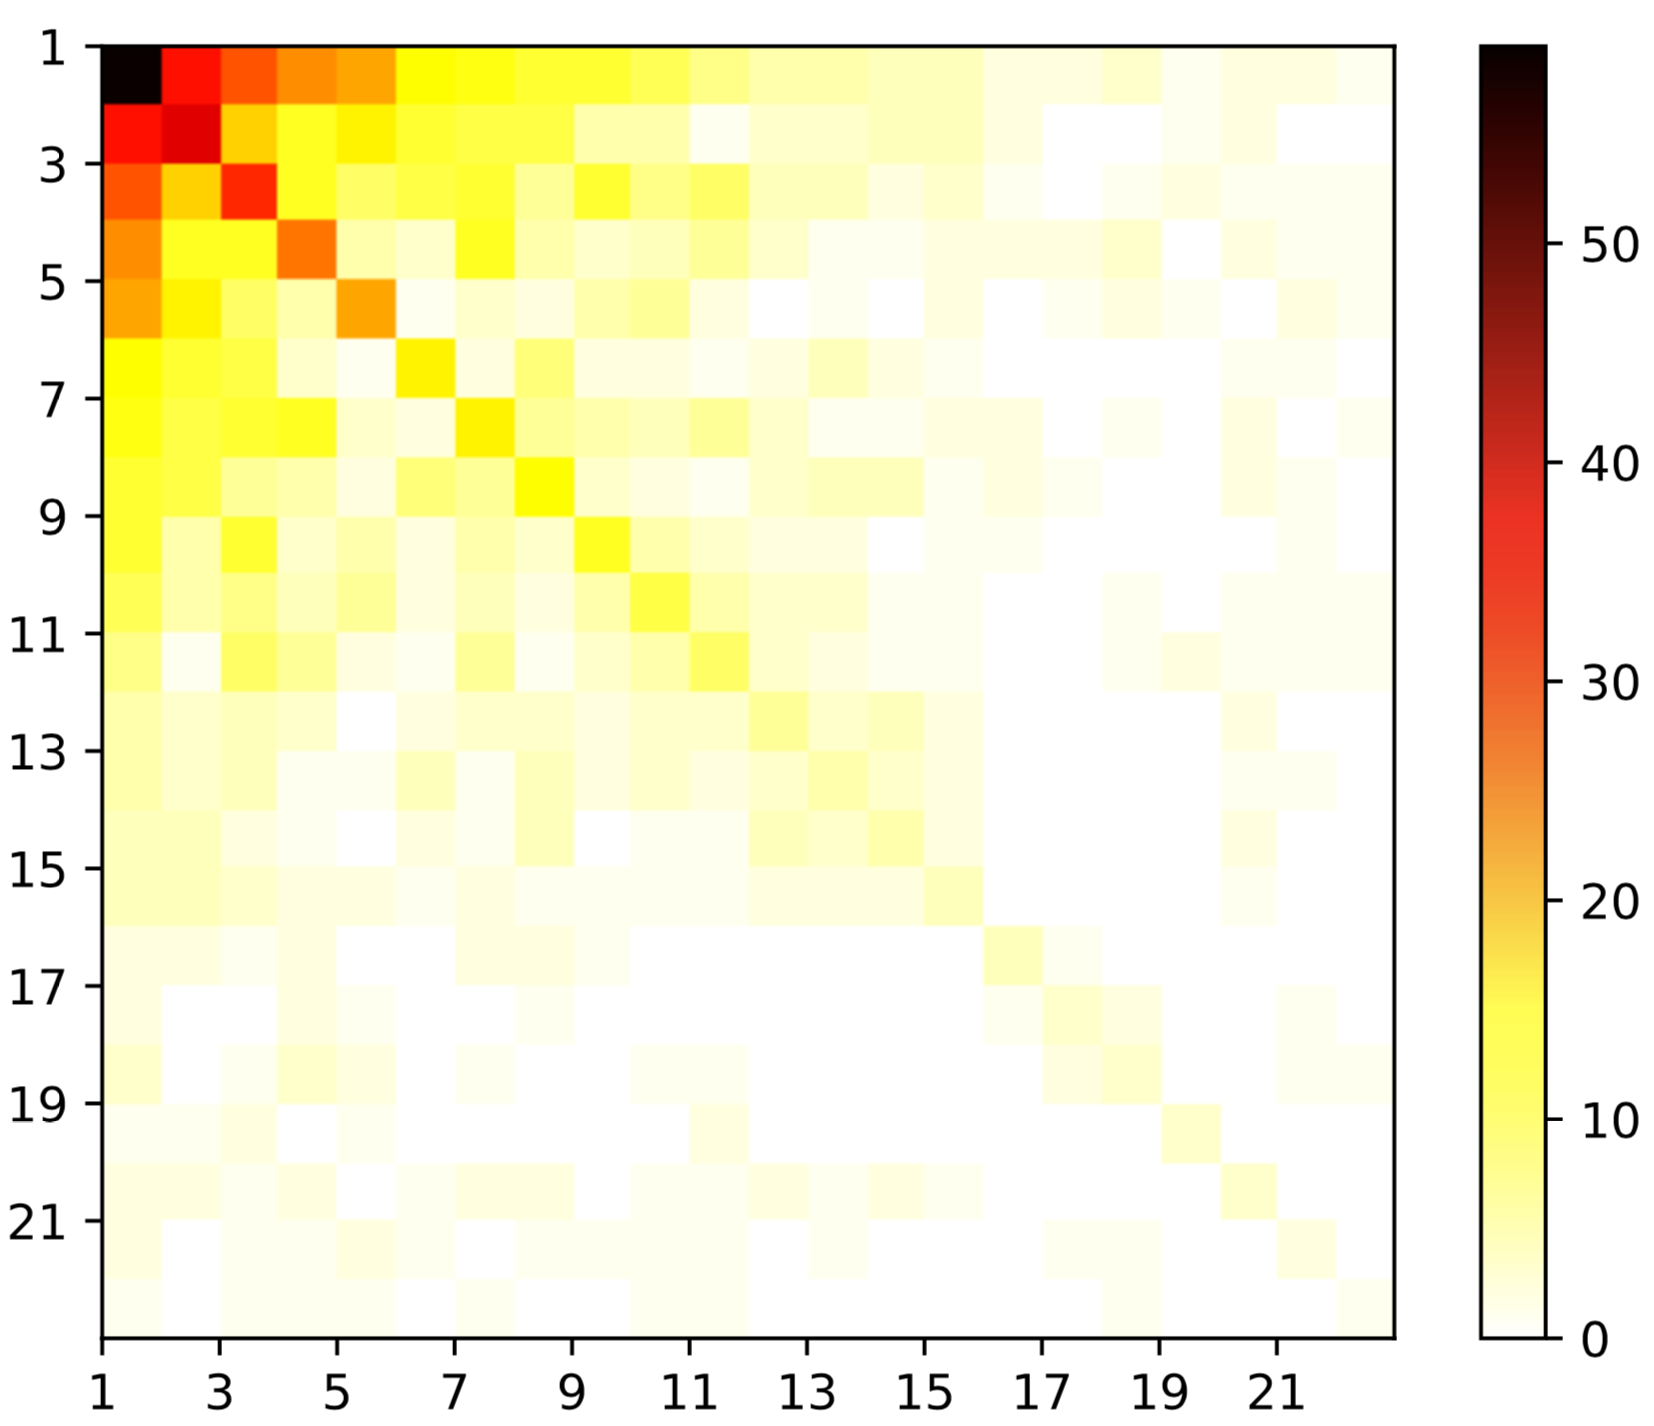
\includegraphics[width=1\textwidth]{img/motivation/tpc-ds-store_sales}
        \caption{The $store\_sales$ table in TDC-DS.}
        \label{fig:ds_count_cdf}
    \end{subfigure}%

    \begin{subfigure}[t]{0.5\textwidth}
        \centering
        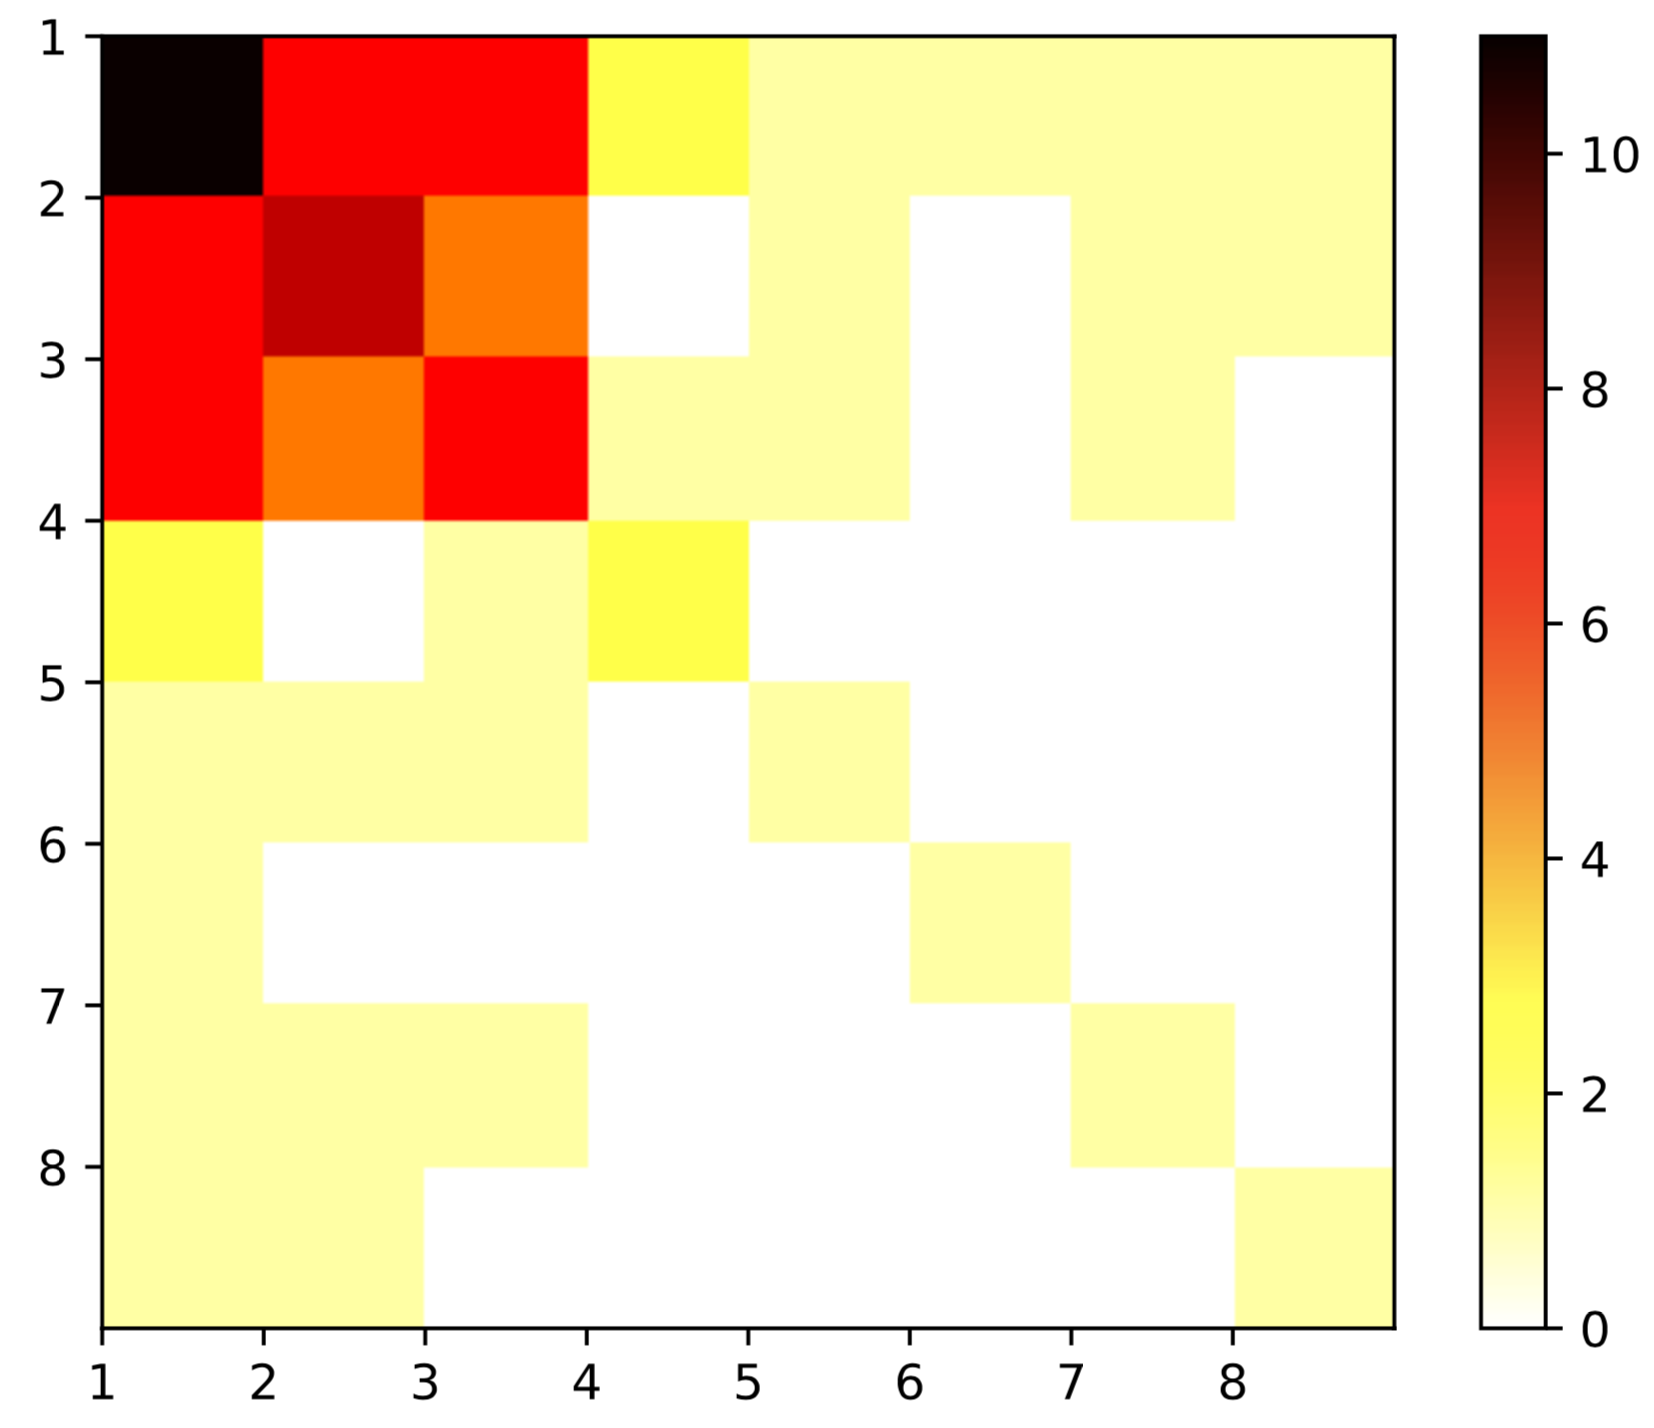
\includegraphics[width=1\textwidth]{img/motivation/tpc-h-orders}
        \caption{The $orders$ table in TDC-H.}
        \label{fig:h_count_cdf}
    \end{subfigure}%

    \begin{subfigure}[t]{0.5\textwidth}
        \centering
        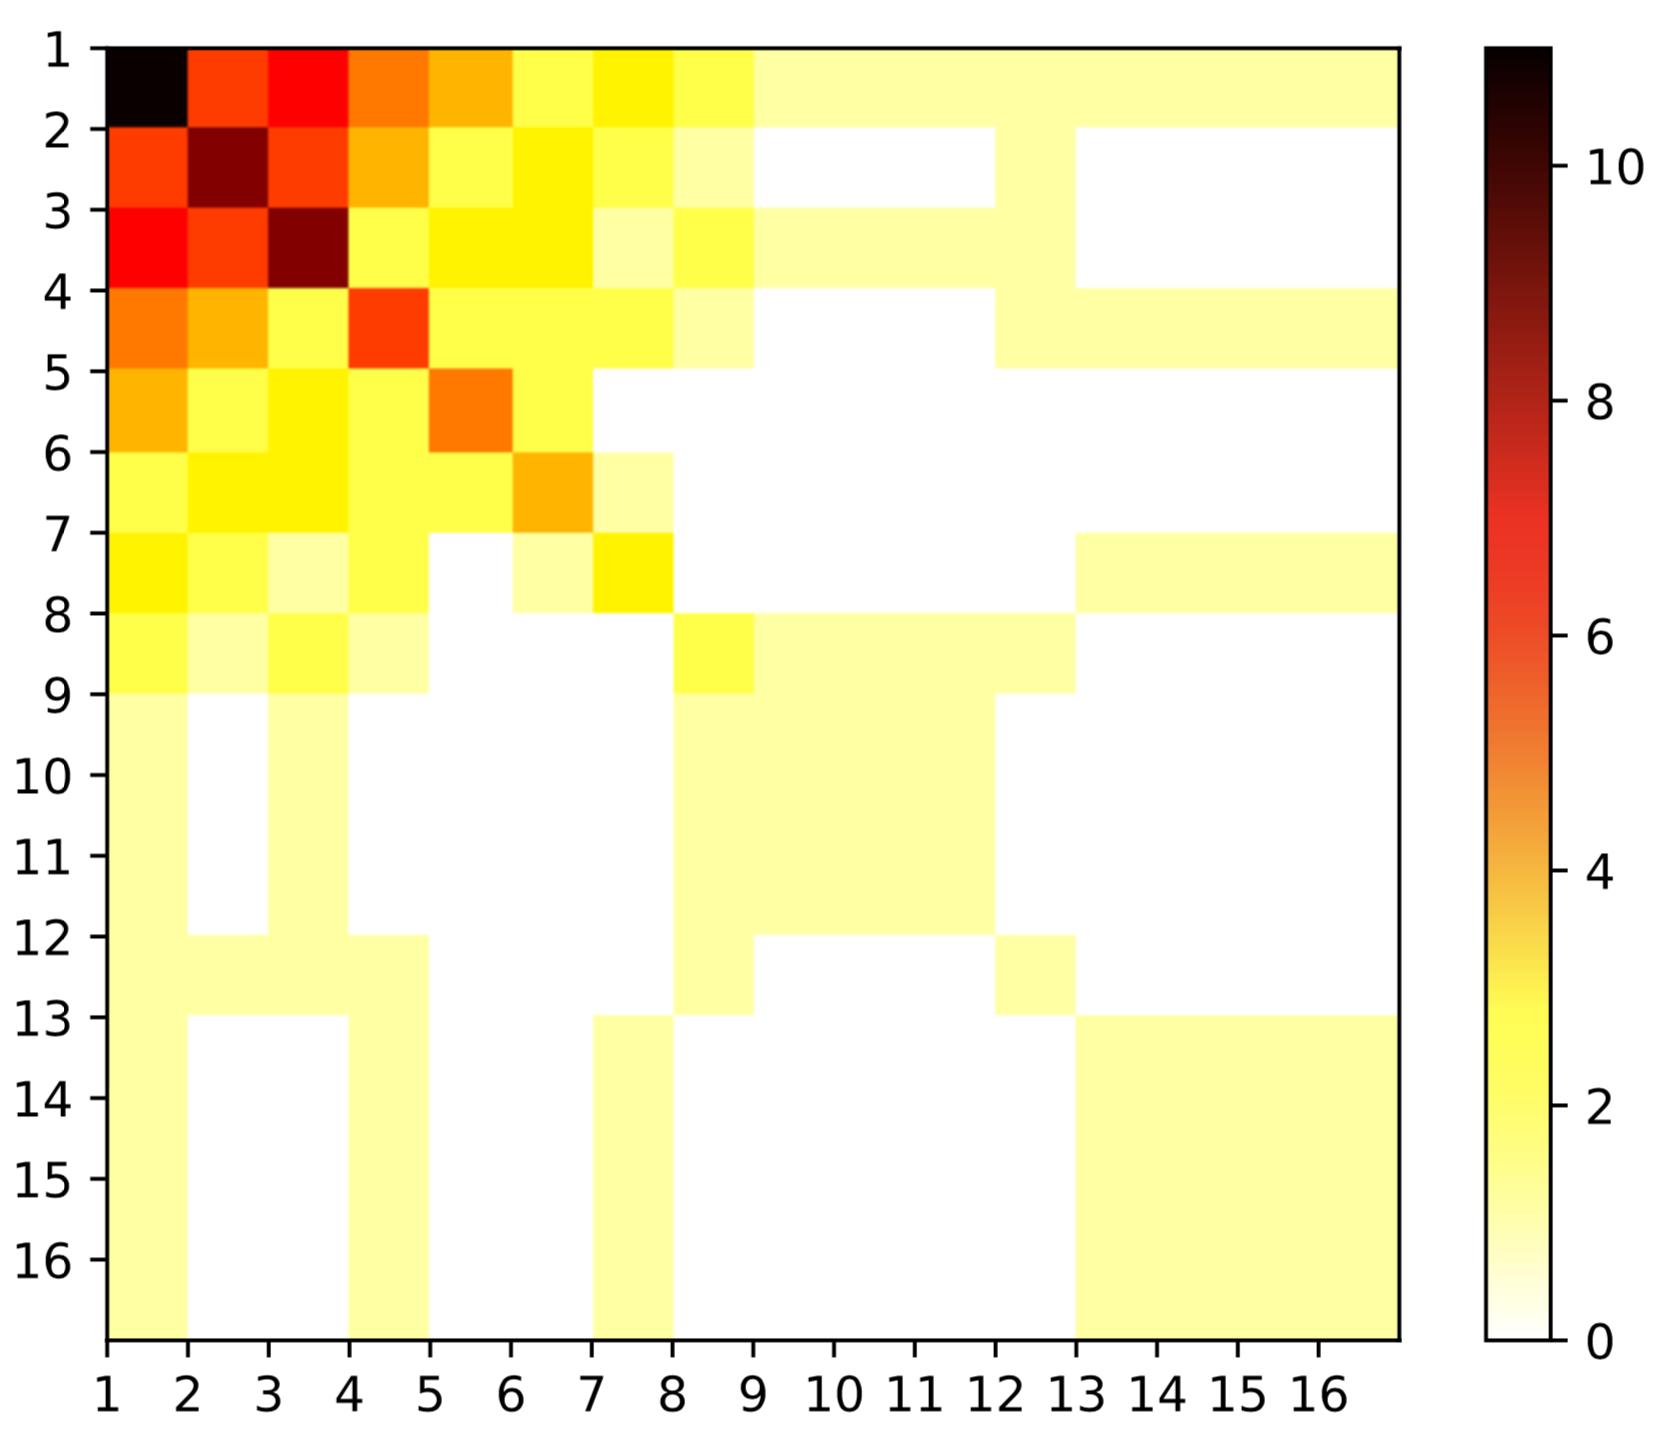
\includegraphics[width=1\textwidth]{img/motivation/tpc-bb-store_sales}
        \caption{The $store\_sales$ table in TDC-xBB.}
        \label{fig:bb_count_cdf}
    \end{subfigure}%
    \caption{Access heat maps of representative tables in the three benchmarks.}
    \label{fig:heatmap}
    %\vspace{-.1in}
\end{figure}

\section{列之间的数据shuffle}
\label{sec:data-shuffle}

\par 从~\ref{sec:col-access}节中观察到的现象我们获悉,每张数据表中一小部分的列非常热门,访问频率很高。如果我们复制这一小部分热门的列,并将它们缓存在不同的机器上,那么当SQL查询任务在分布式环境中执行时,这些热门的列很容易引起集群节点之间的数据shuffling。我们推测,这种shuffling给任务执行时间带来的影响是不可忽视的,为了展示列这一级别的网络开销,我们做了一个实验,测量一个小集群中列的热门程度与数据shuffling的关系。

\subsection{实验设置}
\label{subsec:data-shuffle-setup}

\par 我们部署了一个含有1个master和2个worker的小集群,所用的实例是c5.4xlarge,每一个有32 GB内存和16个CPU核,通过iperf3测试,小集群的网络带宽是10 Gbps。我们在集群上部署了Alluxio以及Spark,运行TPC-H标准测试程序。在实验中,只有一台worker缓存有6 GB的Parquet格式的数据,因此集群里每次执行查询任务都会引发从有数据的机器到没有数据的机器的数据shuffling。我们关闭了Spark和Alluxio的数据被动缓存功能,一个一个按顺序执行标准测试程序里的查询任务,保证每一次执行都会有数据shuffling。我们会记录每一列的总shuffle量。

\begin{figure}[]
	\centering
	\begin{subfigure}[t]{0.5\textwidth}
		\centering
		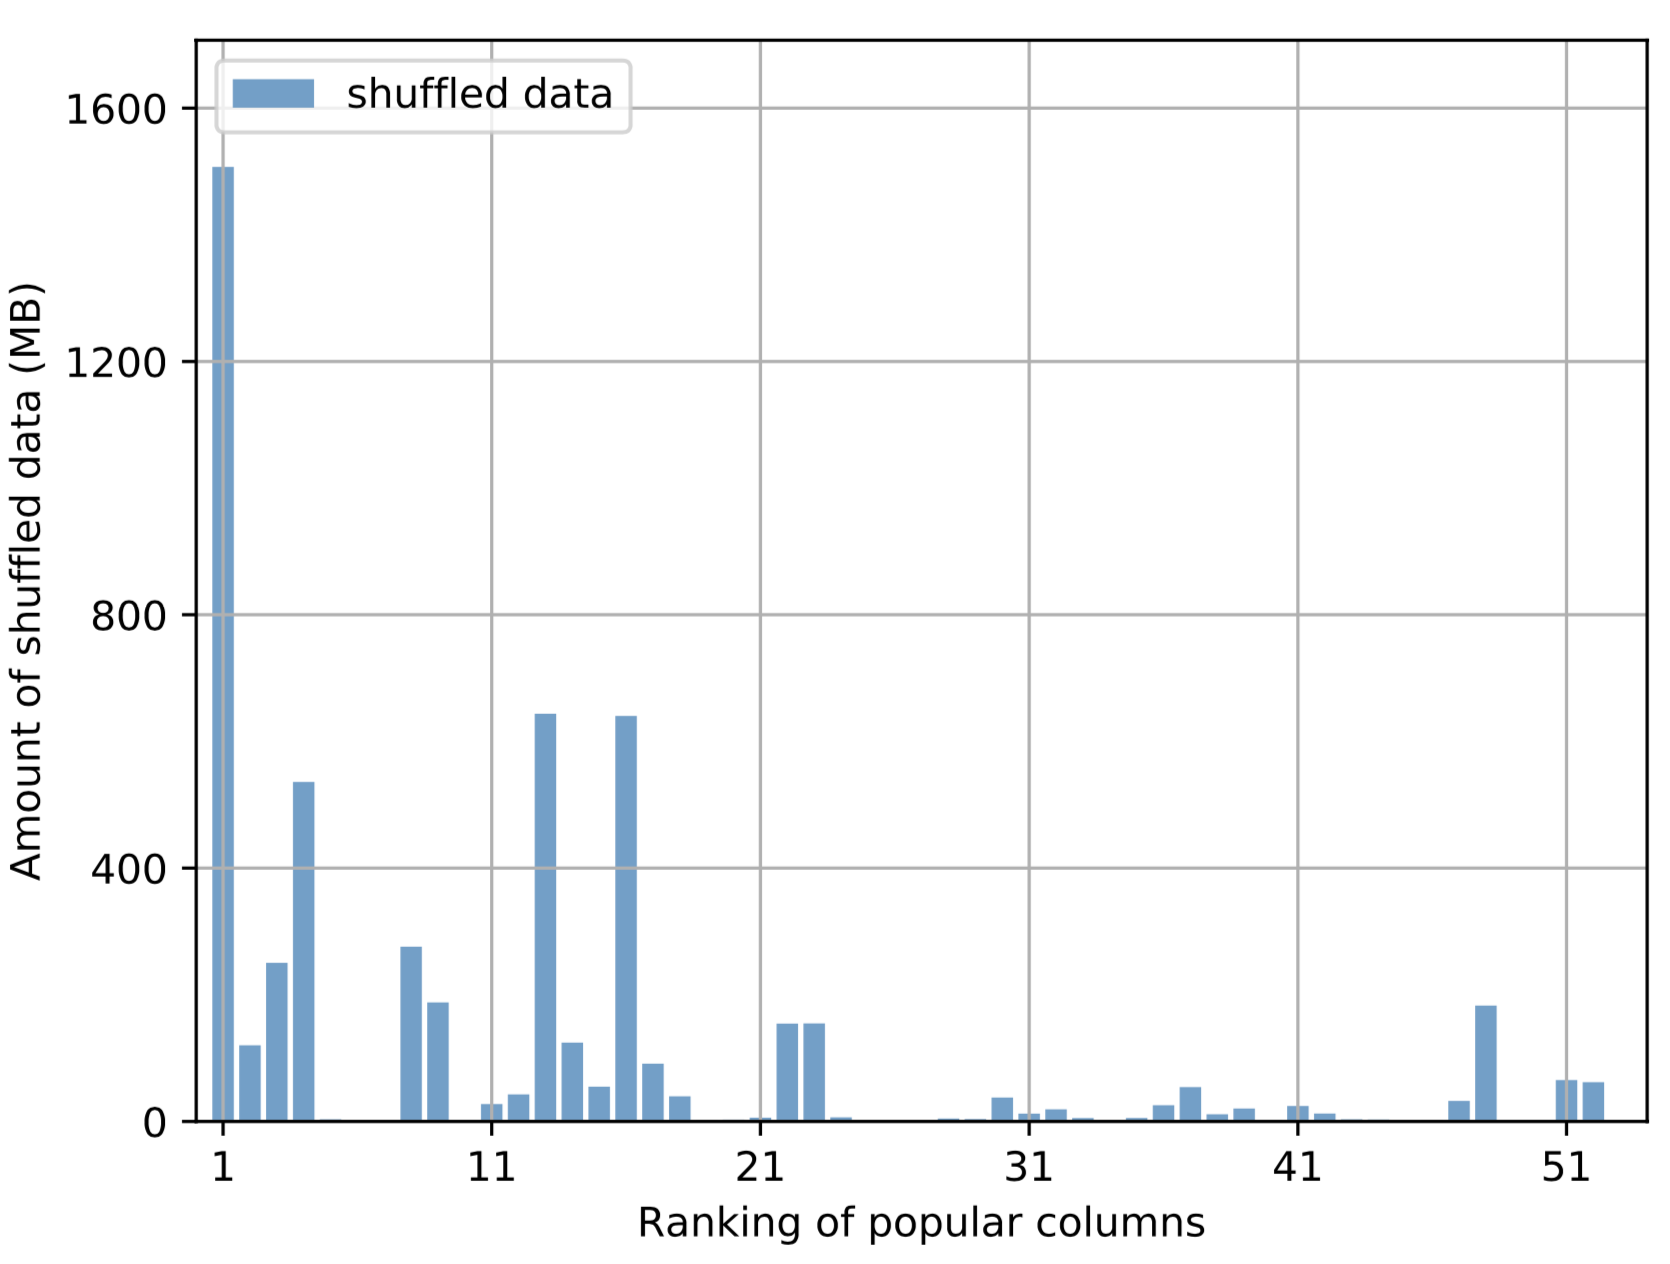
\includegraphics[width=1\textwidth]{img/motivation/pop-shf-a}
		\caption{每一列的总shuffle数据量。}
		\label{fig:pop-shf-a}
	\end{subfigure}%
	
	\begin{subfigure}[t]{0.5\textwidth}
		\centering
		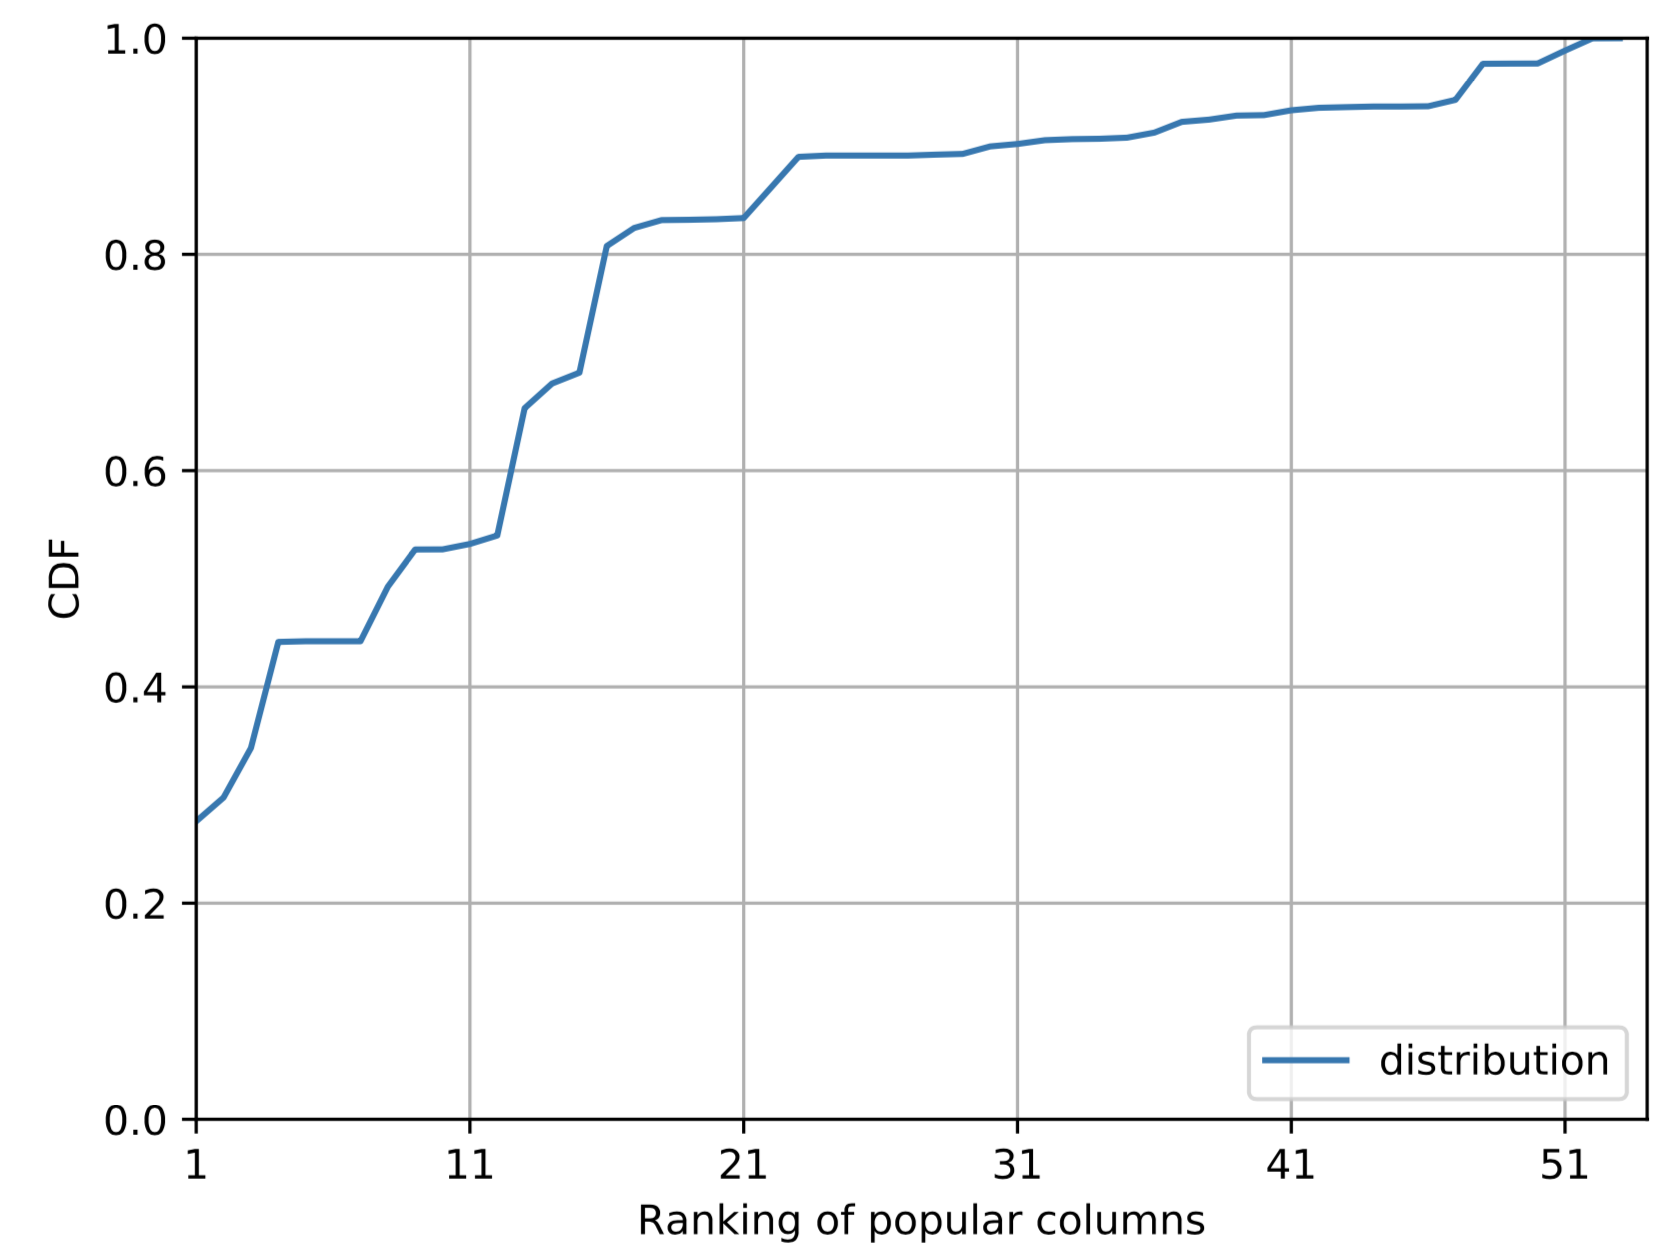
\includegraphics[width=1\textwidth]{img/motivation/pop-shf-b}
		\caption{列级别shuffle数据的CDF。}
		\label{fig:pop-shf-b}
	\end{subfigure}%
	
	\caption{TPC-H标准测试程序的列级别数据shuffle。}
	\label{fig:pop-shf}
	%\vspace{-.1in}
\end{figure}

\subsection{每一列的数据shuffle}

\par 图~\ref{fig:pop-shf}展示了上述实验的结果,其中图~\ref{fig:pop-shf-a}展示了列级别的数据shuffle量,TPC-H标准格式程序中53列按照它们的热门程度排序。因为热门的列被频繁访问,并且我们发现通常来说热门的列比冷门的列的体积更大,所以热门的列相比冷门的列引起更多的数据shuffle。根据图~\ref{fig:pop-shf-b}展示的分布,总体来说,查询任务产生的数据shuffle主要来自热门的列,比如接近90\%的数据shuffle量是由30\%最热门的列贡献的。

\section{数据shuffle的影响}
\label{sec:shuffle-impact}

\par ~\ref{sec:data-shuffle}节实验证明了热门的列很容易引起数据shuffle,本节中我们会用实验证明数据shuffle会降低执行查询任务的性能。

\subsection{实验设置}
\label{subsec:shuffle-impact-setup}

\par 这个实验所用的集群与~\ref{subsec:data-shuffle-setup}小节中描述的集群一致。我们设置了对照实验,其中实验组的设置与~\ref{subsec:data-shuffle-setup}小节一致,只把数据缓存在一台worker上,这一组会产生数据shuffle;另外一组中,我们将相同的数据在两台worker上均进行缓存,保证不会产生数据shuffle。我们对比两组中查询任务的执行时间,以此测量shuffle的开销。

\subsection{度量指标}
\label{subsec:shuffle-impact-metrics}

\par 我们使用任务的平均执行延迟\emph{slowdown}作为衡量指标:
\begin{equation}
    \text{Slowdown} = \frac{L_S - L_N}{L_N},
    %\text{Slowdown} = \frac{L_S - L_N}{L_N} \times 100\%,
\end{equation}

\par 其中$L_S$ 和 $L_N$ 分别是由shuffle和没有shuffle的实验中查询任务的执行时间。\emph{slowdown}的值越大表明其降低查询任务执行的性能的影响越显著。

\subsection{不同网络带宽下的shuffle开销}

\par 按照~\ref{subsec:shuffle-impact-setup}小节的设定,我们依次执行了TPC-H标准测试程序提供的查询任务并计算了每个查询任务的\emph{slowdown}(~\ref{subsec:shuffle-impact-metrics})。图~\ref{fig:cdf16-all}展示了网络带宽被限制为1 Gbps,3 Gbps和10 Gbps的情况下,\emph{salowdown}的分布。从图中可以看出,对于分布式环境下执行的SQL查询任务,网络是瓶颈,所以数据shuffle大大影响了任务执行的性能。例如,即便是在10 Gbps的带宽下,40\%的查询任务的延迟由于数据shuffle会上升10\%。此外,当网络带宽变得越小,shuffle带来的通信开销会更加明显,任务的性能的下降也会更加显著。



\begin{figure}[]
	\centering
	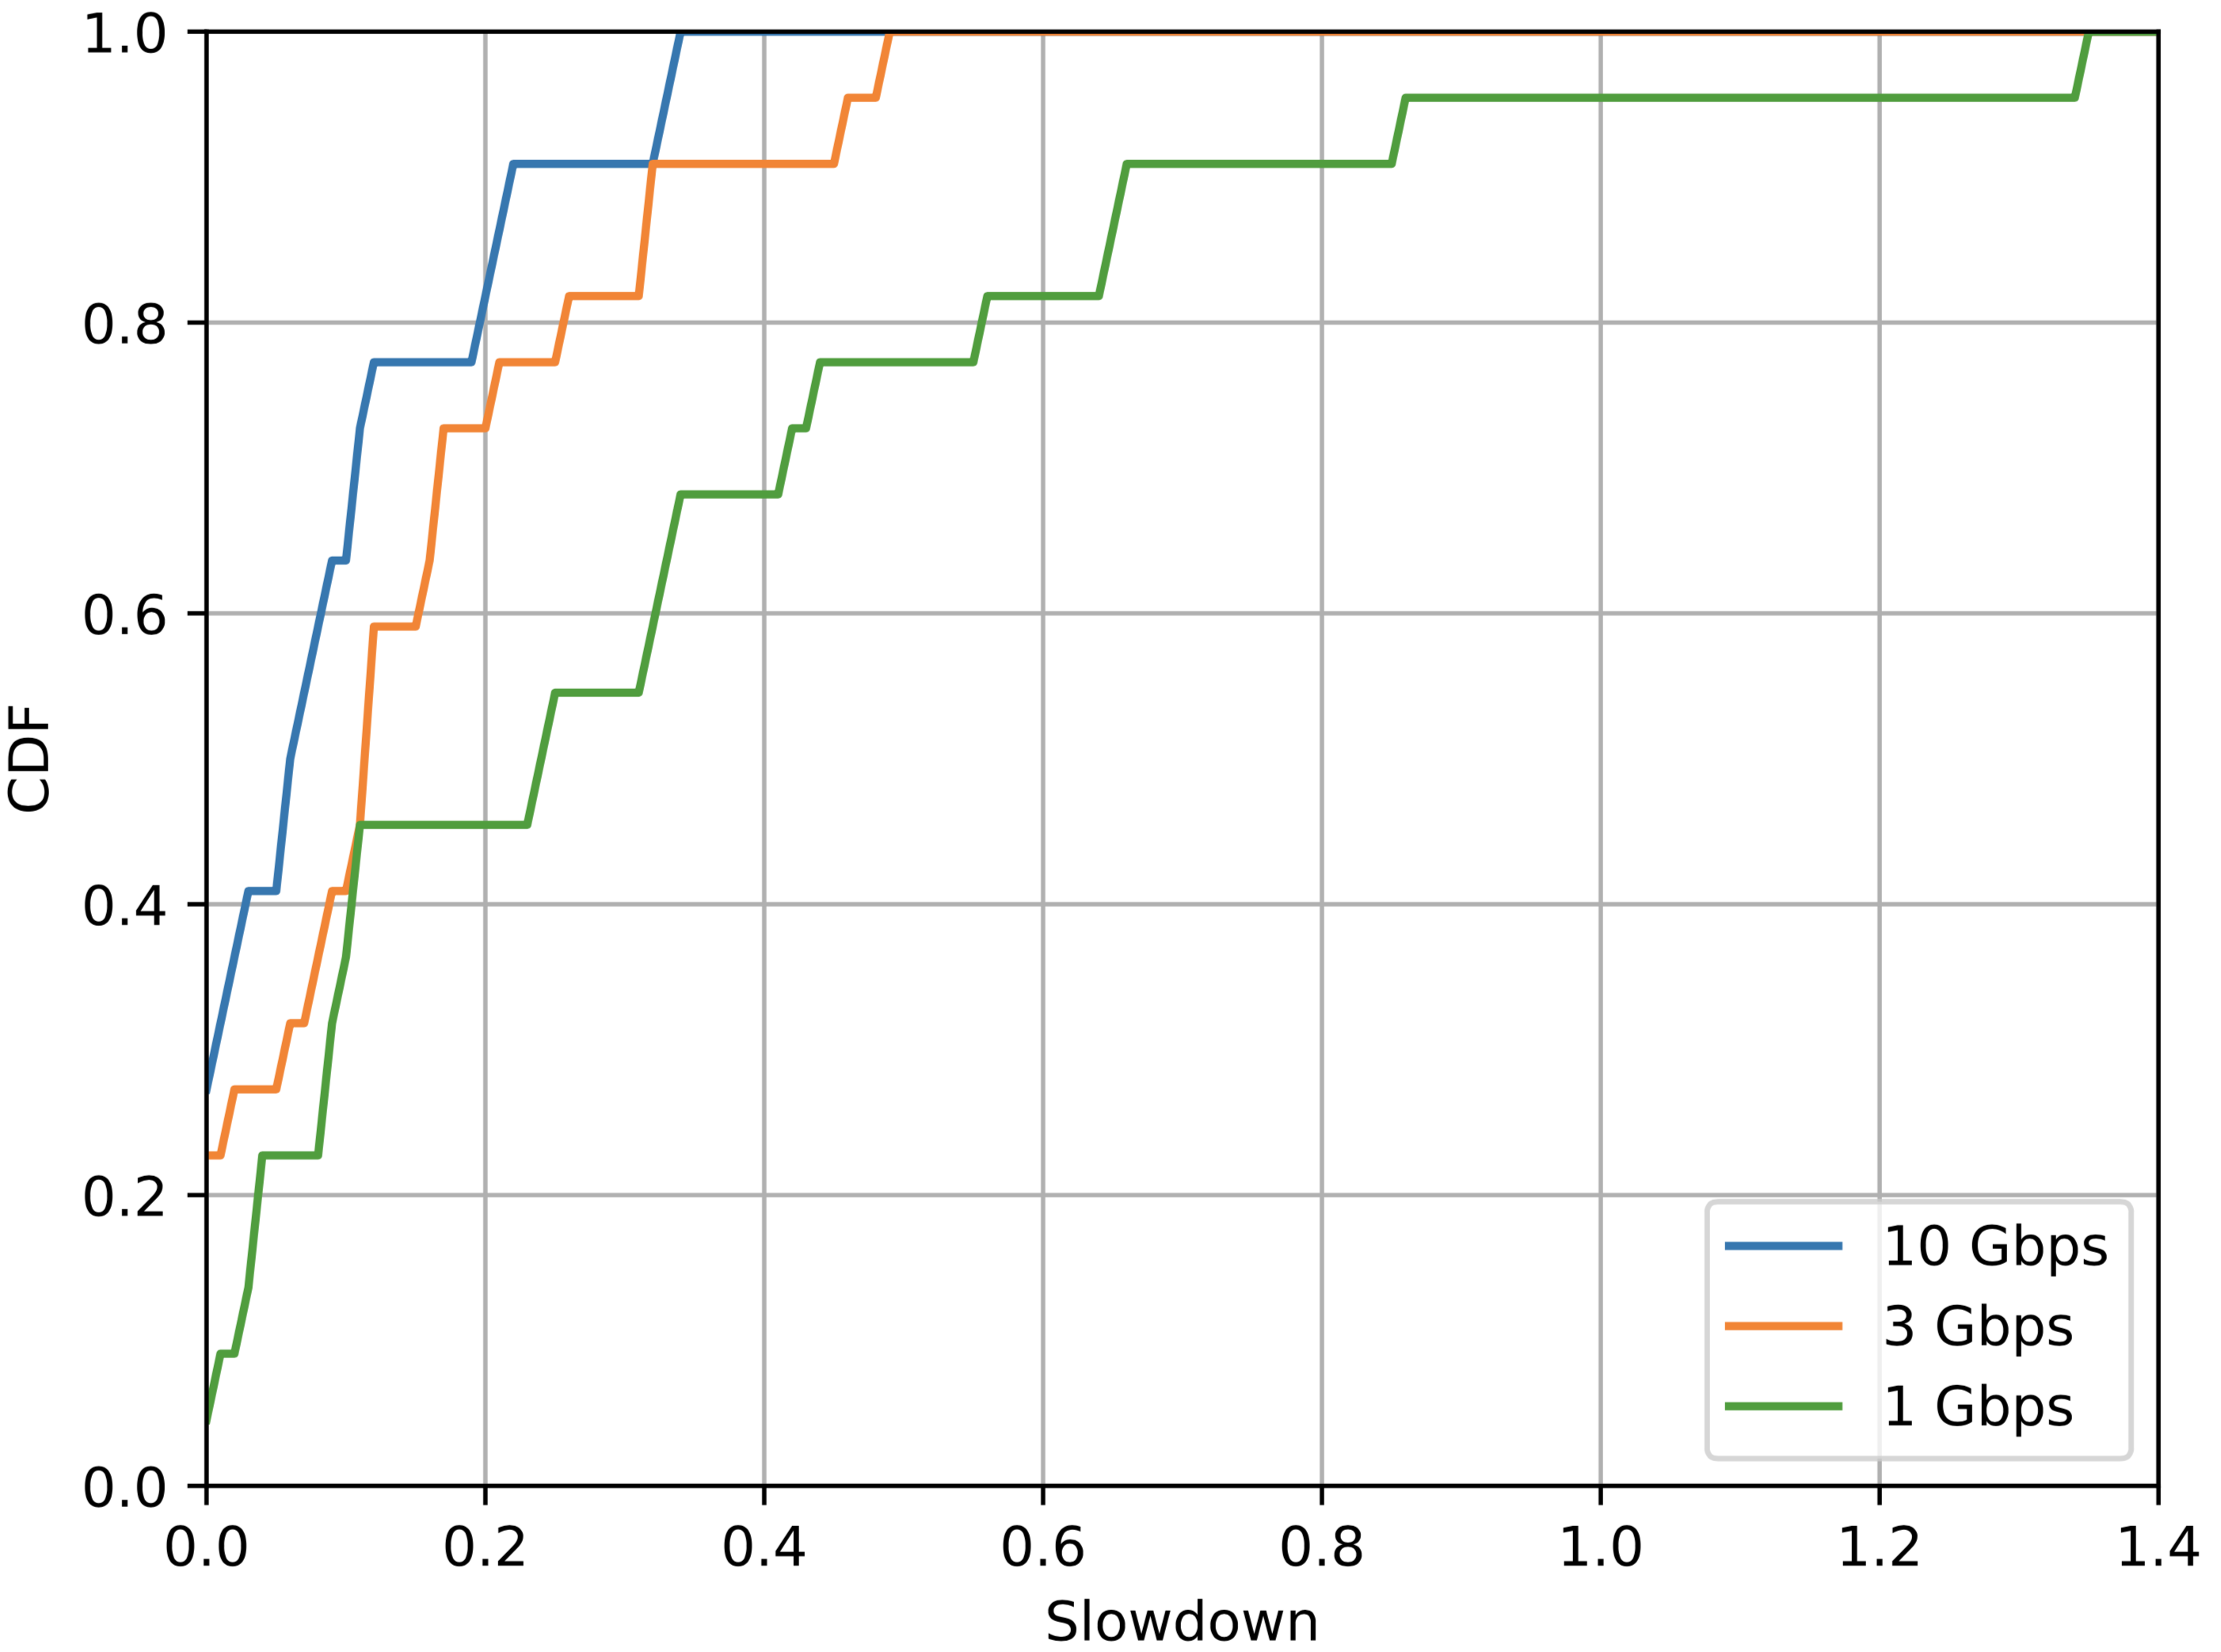
\includegraphics[width=0.5\textwidth]{img/motivation/cdf16-all}
	
	\caption{slowdown在不同网络带宽下的分布。}
	\label{fig:cdf16-all}
	%\vspace{-.1in}
\end{figure}

\section{总结}

\par 我们从本章第~\ref{sec:col-access}节得知,一张数据表中不同列之间热门程度(访问频率)存在明显的差异,且当考虑两两之间被共同访问的概率时,两列的热门程度越高,二者被共同访问的频率越高。在一张表中,热门的列是少数,其余多数是冷门的,不经常被访问。我们这些规律可以推断,相比对整张数据表进行复制,理论上复制数据表里相对热门的若干列能够达到接近复制整表的负载均衡的效果。因为冷门的列本身访问次数不多,在较长的一段周期内,热门的列的访问负载由其副本承担,而冷门的没有被复制的列的访问负载由原表承担,直观来说,这能够起到不错的负载均衡效果。与此同时,复制更少的列,降低缓存开销。提高缓存效率。

\par 将热门的列分别复制,如果随机放置在缓存服务器上,那么一个查询任务很容易引起表内部的数据shuffle,因为各个列的副本很有可能不在同一台服务器上。第~\ref{sec:data-shuffle}节显示,通常来说,热门的列引起的数据shuffle的量更大,第~\ref{sec:shuffle-impact}节证明,表内部的数据shuffle对于查询任务的执行时间的影响是不可小觑的。

\par 以上总结告诉我们,设计方案时我们需要考虑:第一,哪些列是热门的列,需要复制多少热门的列;第二,复制以后,这些列在集群里如何放置,这涉及到“捆绑”(bundle)放置的问题。